\documentclass[pdftex,12pt,a4paper]{article}

\usepackage{graphicx}  
\usepackage[margin=2.5cm]{geometry}
\usepackage{breakcites}
\usepackage{indentfirst}
\usepackage{pgfgantt}
\usepackage{pdflscape}
\usepackage{float}
\usepackage{epsfig}
\usepackage{epstopdf}
\usepackage[cmex10]{amsmath}
\usepackage{stfloats}
\usepackage{multirow}

\renewcommand{\refname}{REFERENCES}
\linespread{1.3}

\usepackage{mathtools}
%\newcommand{\HRule}{\rule{\linewidth}{0.5mm}}
\thispagestyle{empty}
\begin{document}
\begin{titlepage}
\begin{center}
\textbf{}\\
\textbf{\Large{ISTANBUL TECHNICAL UNIVERSITY}}\\
\vspace{0.5cm}
\textbf{\Large{COMPUTER ENGINEERING DEPARTMENT}}\\
\vspace{2cm}
\textbf{\Large{BLG 242E\\ DIGITAL CIRCUITS LABORATORY\\ HOMEWORK REPORT}}\\
\vspace{2.8cm}
\begin{table}[ht]
\centering
\Large{
\begin{tabular}{lcl}
\textbf{HOMEWORK NO}  & : & 1 \\
\textbf{LAB SESSION}  & : & FRIDAY - 16.30 \\
\textbf{GROUP NO}  & : & 18 \\
\end{tabular}}
\end{table}
\vspace{1cm}
\textbf{\Large{GROUP MEMBERS:}}\\
\begin{table}[ht]
\centering
\Large{
\begin{tabular}{rcl}
150200916  & : & Denıs Iurıe Davıdoglu \\
150220770  & : & Onur Baylam \\
\end{tabular}}
\end{table}
\vspace{2.8cm}
\textbf{\Large{SPRING 2023}}

\end{center}

\end{titlepage}

\thispagestyle{empty}
\addtocontents{toc}{\contentsline {section}{\numberline {}FRONT COVER}{}}
\addtocontents{toc}{\contentsline {section}{\numberline {}CONTENTS}{}}
\setcounter{tocdepth}{4}
\tableofcontents
\clearpage

\setcounter{page}{1}

\section{INTRODUCTION [10 points]}

In this homework, preliminary part revises basic digital circuits topics, such as 2's complement notation; minimization of logic functions using 
Karnaugh diagram and Quine-McCluskey method; implementing the same function with different logic components, such as universal NAND gates, multiplexer, decoder. In the experiment part, basic logic circuits are implemented and simulated in Verilog HDL, in the order of increasing complexity, with the final module being 16-Bit Adder-Subtractor.

\section{MATERIALS AND METHODS [40 points]}



\subsection{FIRST HEADER}
$ F_1 (a, b, c, d) = \cup_1 (0, 2, 6, 7, 8, 10, 11, 15) + \cup_{\phi} (4)$

$F_2 (a, b, c) = \overline{a}bc + a\overline{b}c$

$F_3 (a, b, c) = ab\overline{c} + ab$
	
\begin{figure}[ht]
    \centering
	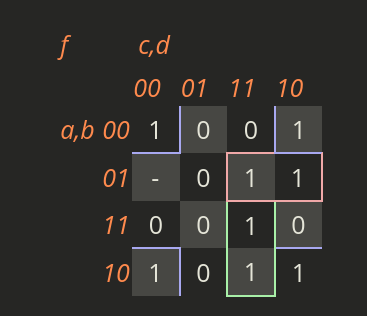
\includegraphics[width=0.5\textwidth]{map1.png}	
	\caption{Karnaugh map of the function  f\cite{ref1}}
	\label{fig1}
\end{figure}

\subsection{SECOND HEADER}


\section{RESULTS [15 points]}
Give the your results what did you get during the experiment. You can also add table, image, etc. 

\section{DISCUSSION [25 points]}
Please explain, analyze, and interpret what have you done during the  experiment. 

\section{CONCLUSION [10 points]}
Comment on any difficulties you have faced, what you have learned etc.

\newpage
\addcontentsline{toc}{section}{\numberline {}REFERENCES}

\bibliographystyle{unsrt}
\bibliography{reference}

\end{document}

